\documentclass[a4paper,11pt]{amsart}
\usepackage{geometry}
\geometry{left=2cm,right=2cm,top=3cm,bottom=2cm}
\usepackage{amssymb,amsthm,amsfonts,extarrows}
\usepackage[colorlinks]{hyperref}
\usepackage{graphicx}
\usepackage{tikz-cd}
\renewcommand{\qed}{\hfill\ensuremath{\clubsuit}}
\DeclareMathOperator{\Sp}{Sp}
\DeclareMathOperator{\id}{id}
\DeclareMathOperator{\gl}{GL}
\DeclareMathOperator{\Orth}{O}
\theoremstyle{plain}
\newtheorem*{fact}{Fact}
\newtheorem{lemma}{Lemma}[subsection]
\theoremstyle{theorem}
\newtheorem{prop}{Proposition}[subsection]
\newtheorem{thm}{Theorem}[subsection]
\theoremstyle{definition}
\newtheorem{defn}{Definition}[subsection]
%%%
\title{Symplectic Group and Maslov index}
\begin{document}
	\maketitle
\section{Introduction}
Our goal in this talk is to give the definition of Maslov index for period solution and compare it with Fredholm index defined before. At first, we need to clarify some essential properties of symplectic groups and they are in both algebraic and topology aspects. This provides us possibility of defining Maslov index associated with a path in symplectic group $\Sp(2n)$ and it is homotopy invariant. Roughly speaking, Maslov index is defined for elements of fundamental group of $\Sp(2n)$. Next, we will explain how to guarantee a path in symplectic group for a period solution of hamilation
\section{Basic Properties of Symplectic Group}
Fixed positive integer $n$, we have canonical $\mathbb{R}$-linear isomorphism $\mathbb{R}^{2n} \cong \mathbb{C}^n$ as follows
\[
(x_1, \cdots, x_n, y_1 \cdots, y_n) \mapsto (x_1 + i y_i, \cdots , x_n + iy_n)
\]
This gives natural almost complex structure $J_0$ for $\mathbb{R}^{2n}$, it just sends $x$ to $ix$. It also induces symplectic form $\omega$ as
\[
(v, w) = \omega(v,J_0 w)
\]
since $J_0^2 = -\id$. In this way, $(\mathbb{R}^{2n},\omega)$ is kind of symplectic manifold of dimension $2n$.
Let's consider general linear transformation $A \in \gl(2n,\mathbb{R})$. If $A$ is compatible with symplectic form $\omega$ of $\mathbb{R}^{2n}$, i.e., 
\[
\omega(A v, Aw) = \omega(v,w)
\]
or as matrices
\[
A^{t}J_0 A = J_0
\]
Then we say $A$ is a symplectic matrix. All symplectic matrices of dimension $2n$ form a group called symplectic group in dimension $2n$, denoted by $\Sp(2n)$.
\begin{prop}
	We have following equalities\[
	\Sp(2n) \cap \Orth(2n) = \Sp(2n) \cap \gl(n,\mathbb{C}) = \Orth(2n) \cap \gl(n,\mathbb{C}) = U(n)
	\]
\end{prop}
\begin{fact}
	$U(n)$ is maximal compact subgroup of $\Sp(2n)$ and matrix $A \in \Sp(2n)$ has polar decomposition of form
	\[
	A = US
	\]
	where $S= \sqrt{A^t A}$ and $U= A S^{-1}$. It is easy to see that $U$ is unitary matrix and $S$ is symmetric positive symplectic matrix. Futhermore, this decomposition gives continuous map
	\[
	\begin{aligned}
	\Sp(2n) & \to U(n) \times C_n\\
	A & \mapsto (U,S)\\
	\end{aligned}
	\]
	where $C_n$ is open subset of $\gl(n,\mathbb{C})$ consists of symmetric positive definite symplectic matrices. This map is actually homeomorphism.
\end{fact}
\begin{fact}
	If $A \in \Sp(2n)$, then $ A^{-1} \sim A^t \sim A$.
\end{fact}
With the symplectic condition $A^t J_0 A = J_0$, we have
\[
A^t = J_0 A^{-1} J_0^{-1}
\]
Hence $A^t \sim A^{-1}$. 
Furthermore, we have 
\[
A = -J_0 (A^{-1})^t J_0
\]
Hence
\[
\begin{aligned}
\det(A-\lambda \id)& = \det(-J_0 (A^{-1})^t J_0 -\lambda \id)\\
& = \det (-(A^{-1})^t + \lambda \id)\\
& = \det((A^{-1})^t) \det(\lambda A^t - \id)\\
& = \det((A^{-1})^t)\lambda^{2n} \det( A - \frac{1}{\lambda} \id)
\end{aligned}
\]
This implies that $\lambda$ has same multiplicity of $\lambda^{-1}$ in characteristic polynomial of $A$.
\subsection{Connectivity}
In this section, we plan to prove that $\Sp(2n)$ is connected Lie group, and its fundamental group is isomorphic to $\mathbb{Z}$. It follows that if $\lambda$ is eigenvalue of $A$ then $\lambda^{-1}$ is also. 
\begin{proof}
	We only need to prove $C_n$ is contractible since $\Sp(2n) \simeq U(n) \times C_n$. Let $A \in C_n$, since $A$ is symmetric and symplectic, we can find suitable symplectic basis ( which compatible with it symplectic structure) for $\mathbb{R}^{2n}$ that $A$ is diagonal. We have already known that if $\lambda$ is eigenvalue of $A$, then $\lambda^{-1}$ is too. Hence $A$ is diagonal matrix with blocks like
	\[
	\begin{pmatrix}
	\lambda& & & & & \\
	& \ddots& & & & \\
	& & \lambda & & &   \\
	& & & \lambda^{-1} & & \\
	& & & & \ddots & \\
	& & & & & \lambda^{-1}\\
	\end{pmatrix}
	\]
	Write diagonal matrix $\log A$ with blocks
	\[
	\begin{pmatrix}
	\log\lambda& & & & & \\
	& \ddots& & & & \\
	& & \log\lambda & & &   \\
	& & & -\log\lambda & & \\
	& & & & \ddots & \\
	& & & & & -\log\lambda\\
	\end{pmatrix}
	\]
	Hence there is retraction from $A$ to identity
	\[
	(A,t) \mapsto \exp (t \log A)
	\]
	Therefore, we can conclude that $C_n$ is contractible open subset and this implies that $\Sp(2n)$ has retract $U(n)$. Hence $\Sp(2n)$ is with same homotopy type of $U(n)$. They are both connected and with fundamental group $\mathbb{Z}$.
\end{proof}
In this proof, we also find that the determinant of a symplectic group is just $1$.
\section{Definition of Maslov index}
In this section, we will give the definition of Maslov index for a path in $\Sp(2n)$ such that the end of the path doesn't have eigenvalue $1$.

Let
\[
\Sp(2n)^* = \big\{A \in \Sp(2n)\big| \det(A-\id) \neq 0 \}
\]
It is open subset of $\Sp(2n)$ because the $\det(A-\id)=0$ is closed condition. And we denote $\mathcal{S}$ the path space of all paths connect identity and elements in $\Sp(2n)^*$ i.e., 
\[
\mathcal{S}= \big\{\gamma\colon I \to \Sp(2n) \big| \gamma(0) \id \text{ and } \gamma(1) \in \Sp(2n)^* \}
\]
where $I$ is the interval $[0,1]$. We have following technical theorem due to Salamon and Zehnder
\begin{thm}
	For every positive integer $n$, there exists a continuous map $\rho \colon \Sp(2n) \to S^1$ such that 
	\begin{itemize}
		\item naturality: If $A' \sim A$, then $\rho(A') = \rho (A)$
		\item product: \[
		\rho(\begin{pmatrix}
		A& 0 \\
		0& B\\
		\end{pmatrix}) = \rho(A) \rho(B)
		\] where $A \in \Sp(2n)$ and $B \in \Sp(2m)$.
		\item determinant: we have $U(n) \subset \Sp(2n)$ and $\rho|_{U(n)} = \det_{\mathbb{C}}$. In particular, we have $\rho(I_{2n}) = 1$                          
		\item normalization: if eigenvalue of $A$ are all real number, then $\rho(A) = (-1)^{m_0/2}$, where $m_0$ is the total multiplicity of $A$'s negative real eigenvalues.
	\end{itemize}
\end{thm}
This theorem tells us even we have no knowledge about explicit form of $\rho$, we can also compute $\rho(A)$ for symplectic matrix $A$ if we know eigenvalues of $A$. We know the path lifting $\alpha$ is unique up to homotopy and $\rho$ induces isomorphism on fundamental group of $\Sp(2n)$ and $S^1$, hence we have following well-defined map
\[
\begin{aligned}
 \Delta &\colon \pi_1(\Sp(2n)) \to \mathbb{R}\\
 &[\gamma] \mapsto \frac{\alpha(0) -\alpha(1)}{\pi}
\end{aligned}
\]

For path $\gamma$ in $\Sp(2n)$, we have following diagram
\[\begin{tikzcd}
	& & & \mathbb{R} \ar[d,"\pi"]\\
	&I \ar[r,"\gamma"'] \ar[rru,dashed,"\alpha"]& \Sp(2n) \ar[r,"\rho"'] & S^1\\
\end{tikzcd}\]
where $\pi \colon \mathbb{R} \to S^1$ is the universal covering of $S^1$. However, since $\Sp(2n)^*$ is non-connected, for paths with endpoints in $\Sp(2n)^*$, we need following proposition for topological properties of $\Sp(2n)^*$.
\begin{prop}
	$\Sp(2n)^*$ has two connected components as follows\[
	\Sp^+(2n) = \big\{A \in \Sp(2n)\big| \det(A-\id) > 0 \}
	\]
	and
	\[
	\Sp^-(2n) = \{A \in \Sp(2n)\big| \det(A-\id) < 0 \}
	\] These two components are both simply connected.
\end{prop}
This proposition implies that $\Sp(2n)^*$ is not so bad as topological space (can be decomposed to simply connected parts).

Let 
\[
\begin{aligned}
 W^+ = -I_{2n}& & W^- = \begin{pmatrix}
 2&0 & \\
 0 &\frac{1}{2}& \\
  & &I_{2n-2}\\
 \end{pmatrix}
\end{aligned}
\]
It is not hard to see $W^+ \in \Sp^+(2n)$ and $W^- \in \Sp^-(2n)$. We have following picture for $\Sp(2n)^*$.
\begin{figure}[h]
	\caption{Topology of $\Sp(2n)^*$}
\centering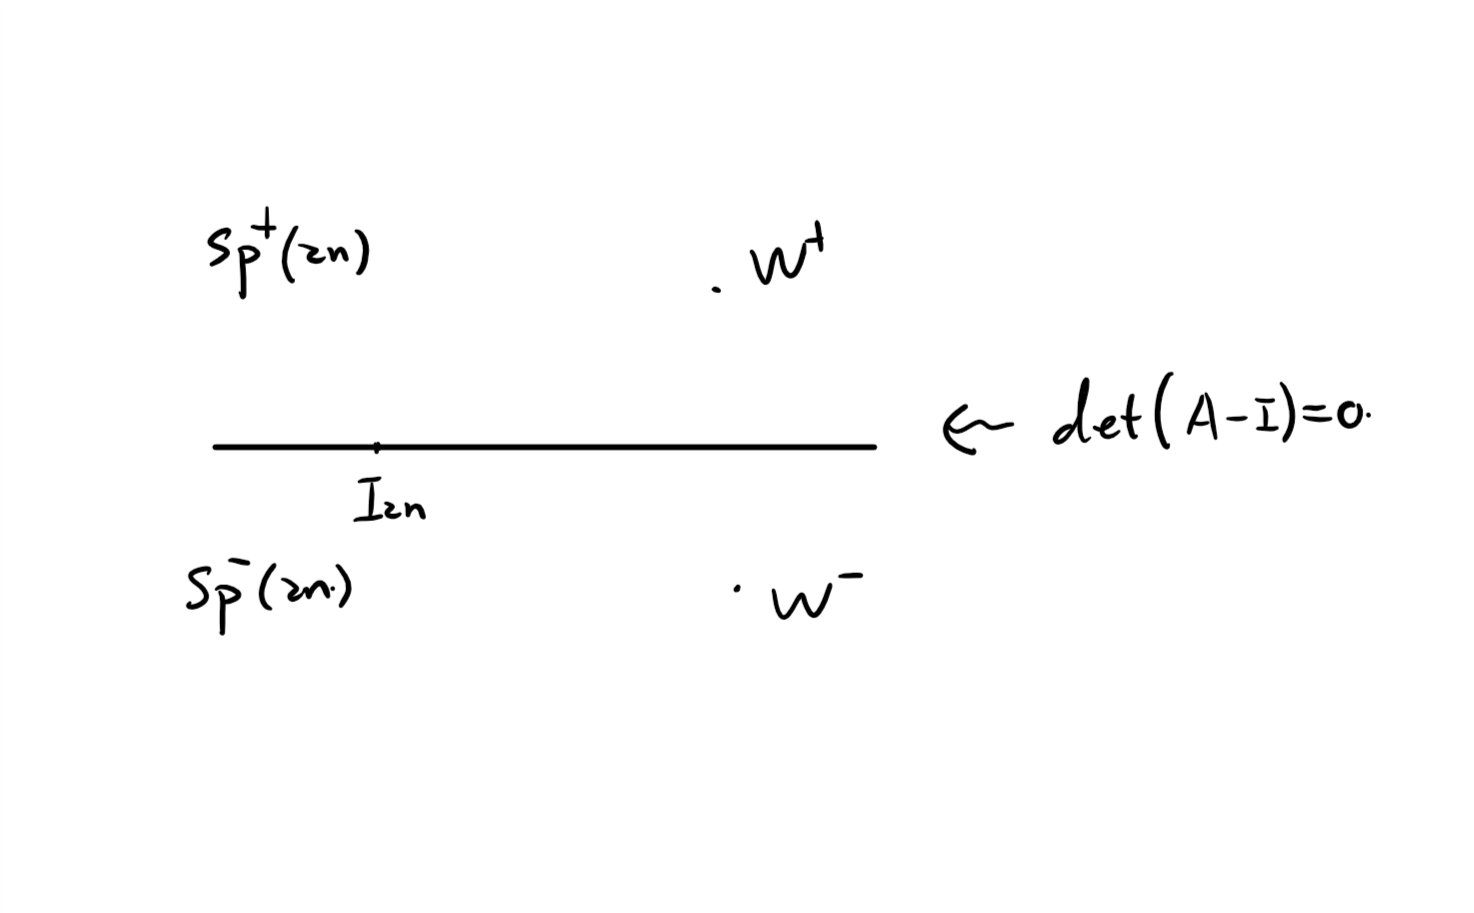
\includegraphics[scale=0.5]{PIC/maslov1.png}
\end{figure}
In order to prove this proposition, we need following technical lemma. We will admit it without proof.
\begin{lemma}
	Let $A \in \Sp(2n)^*$. There exists a path in $\Sp(2n)^*$ that connects $A$ to a matrix $B$ whose eigenvalues are all distinct with exactly zero  ($ A \in \Sp^+(2n)$ )or two ($A \in \Sp^-(2n)$) real positive eigenvalues.
\end{lemma}
Let $B$ be the matrix in upper lemma. Since $B$ has distinct eigenvalues, we can choose suitable symplectic basis for $\mathbb{R}^{2n}$ such that $B$ can be written as diagonal matrix with $2\time2$-blocks like
\[
\begin{pmatrix}
 \lambda & 0 \\
 0 & 1/\lambda\\
\end{pmatrix}
\]
We defined the path start at $B$ in $\Sp(2n)^*$ as $B(t)$ is formed with blocks
\[
\begin{pmatrix}
 \lambda(t) & 0 \\
 0 & 1/\lambda(t)\\
\end{pmatrix}
\]
if $\lambda$ is not positive real eigenvalue of $B$, where $t \mapsto \lambda(t)$ is path connecting $\lambda
$ and $-1$ in $\mathbb{C}$ which avoiding $1$.
If $\lambda$ is positive real eigenvalue, then it is constant along the path.
 
There are two possible cases in the lemma 
\begin{itemize}
	\item If $B$ has no positive real eigenvalue. Then the endpoint $B(1) = -\id$ since all blocks become
	\[
	\begin{pmatrix}
	-1&0\\
	0& -1\\
	\end{pmatrix}
	\]
	\item If $B$ has exactly two real positive eigenvalues. We can switch the basis so that the block os real positive eigenvalues are in the first. Hence the endpoint $B(1)$ is 
	\[
	\begin{pmatrix}
	\lambda &0 & \\
	0 & 1/\lambda& \\
	& & -\id \\
	\end{pmatrix}
	\] 
	We can assume $\lambda > 1$, otherwise switch $\lambda$ and $1/\lambda$. The we can choose a path from $\lambda$ to $2$ avoiding $1$. It enable us to find a path from $B(1)$ to $W^-$.
\end{itemize}
Now we can conclude that each matrix $A \in \Sp^+(2n)$ (resp. $\Sp^-(2n)$) is connected to $W^+$(resp. $W^-$). This implies that both $\Sp^+(2n)$ and $\Sp^{-}(2n)$ are connected component of $\Sp(2n)^*$.

Finally, to show the triviality of the fundamental groups, use following lemma
\begin{lemma}
	There exist continuous $\rho^{\pm} \colon \Sp^{\pm}(2n) \to \mathbb{R}$ such that the diagram commute
	\[
	\begin{tikzcd}
	& \mathbb{R} \ar[dr] & \\
	\Sp^{\pm}(2n) \ar[r,"i_{\pm}"'] \ar[ru,"\rho^{\pm}"]& \Sp(2n) \ar[r,"\rho"]& S^1\\
	\end{tikzcd}
	\]
\end{lemma}
Since $\rho$ induce isomorphism on fundamental group and $\mathbb{R}$ is contractible, we have $i_{\pm}$ induces trivial morphisms on fundamental groups, which means $\pi_1(\Sp^{\pm}(2n))= 0$. 
\qed

Now, we know for $A \in \Sp^{pm}(2n)$ we can choose a path $\gamma_A$ connect $A$ and $W^{\pm}$ and this path is unique up to homotopy. Hence $\Delta(\gamma_A)$ only depends on the choice of $A$. We denote it by $r(A)$. 

This moment, we prepare well for giving the definition of \emph{Maslov index}
\begin{defn}[Maslov index]
Let $\psi \in \mathcal{S}$. The Maslov index of $\psi$ is defined as
\[
 \mu(\psi) = \Delta(\gamma_{\psi(1)} \cdot \psi)= \Delta(\psi) + r(\psi(1))
\]	
\end{defn}
$\rho(I_{2n}) = 1 \in 
S^1$ and $\rho(W^{\pm}) = \pm 1 \in 
S^1$, their fiber on $\mathbb{R}$ is some times of $\pi$, so $\mu(\psi) \in \mathbb{Z}$ for all $\psi \in \mathcal{S}$. This is why we call it index.
\section{The path of orbits}
In this section, we will try to explain how to associate a path $\psi \in \mathcal{S}$ for a non-degenerated 1-period solution $x$. Unfortunately, this explanation will be very rough and we need some extra assumption.
Let $x$ be a 1-period solution of Hamiltonian
\[
H \colon W \times S^1 \to \mathbb{R}
\]
Suppose $\varphi^t$ be the  time-flow of $H$, then $x(t) = \varphi^t(x(0))$. Since $\varphi^t$ preserves symplectic form and $x$ is non-degenerated, we have the tangent map $T_{x(0)}\varphi^1 \in 
\Sp(2n)^*$. In following picture, we show what happened on vector fields of $x$.

To associate a path for solution $x$, we need a trivialization of tangent bundle $x^* TM$ on $S^1$. It means that we need define frame at each point of $S^1$. We have following theorem providing us existence of such trivialization
\begin{thm}
	For every continuous map \[\psi \colon D^k \to W\]
	the symplectic fiber bundle $\psi^* TW$ can be trivialized and all its trivializations are homotopic.
\end{thm} 
Since $x$ is contractible, there is some continuous $u$ extending $x$ on the disk $D^2$, i.e., $u|_{\partial D^2} = x$. Since $u^*TM$ has unique trivialization up to homotopy, hence we get trivialization for $x^*TM$. If there is another extension $v$ of $x$ on $D^2$, we can glue them to a map 
\[
s\colon S^2 \to M
\]
thanks to assumption 6.2.2 that every $C^\infty$-map $s: S^2 \to M$, there exists a symplectic trivialization of the fiber bundle $s^* TM$, and it is unique up to homotopy. Then we get the two trivialization given by $u$ and $v$ are homotopy. Hence we get a well-defined trivialization for fiber bundle $x^*TM$ and it provides us unique path $\psi \in \mathcal{S}$ up to homotopy.
\end{document}